In this chapter, the method used to investigate the problem statement is
presented. First, the choice of method is described, motivating the dataset and
technologies used. Following this the problems used for benchmarking are
presented, including a more in-depth description of the dataset. After these
motivations, the actual implementation details are presented, showing how the
database's are evaluated. Finally the results from the evaluation are presented.

\section{Choice of method}\label{sec:choiceofmethod}
This section will motivate the methods' three primary questions:
\begin{enumerate}
\item What databases are evaluated?
\item What dataset is used to evaluate the databases?
\item How are the databases evaluated?
\end{enumerate}

The following three sections will answer these questions in order, motivating
choice of databases, dataset and implementation.

\subsection{Choice of databases}\label{sec:choiceofdatabases}
The two database chosen to evaluated are PostgreSQL and MariaDB. The choice was
made, as they both are:
\begin{enumerate}
\item Modern databases with widespread use and active development;
\item Open-source projects allowing anyone to read and modify the source code;
\item And they implement state-of-the-art algorithms and methods.
\end{enumerate}

In addition to this they both cover two common use-cases: academia and
enterprises. All research papers mentioned in Chapter~\ref{chap:relatedwork} that have
implemented new algorithms or modified old ones have done so in PostgreSQL.
On the other hand MariaDB is compatible with MySQL, making it a common
alternative for enterprises.

An evaluation of both of these database will give a good indication of the
performance of a modern state-of-the-art query optimizer. Furthermore, as
mentioned in Section~\ref{sec:purpose} since both of them are open-source, if
one performs better than the other the code can be studied to identify areas of
improvement.

\subsection{Choice of dataset}\label{sec:dataset}
The primary focus when selecting the dataset used was to use a dataset which
could capture the complexity of a real-world database and provide a realistic
challenge for the query optimizer. The primary requirements are that the dataset
feature:
\begin{enumerate}
\item Many tables with multiple indexes;
\item Not just indexes on a single row, but also compound indexes covering
  several;
\item Skewed and non-uniform data that is not trivial to correctly estimate
  based on sampling;
\item A large amount of data forcing the database to estimate the data.
\end{enumerate}

The datasets most commonly used for evaluation of database implementations are
TPC-H~\cite{tpc_th}, TPC-DS~\cite{tpc_tha} and more recently
JOB~\cite{leis_2015_how_hgaqor}. None of these datasets however feature the
several indexes on the same table or compound indexes, making the problem of
index selection trivial for all of them.

Instead, the dataset chosen was one taken from the real world: the dataset for
TriOptima's product TriReduce. This database fulfill all of the requirements, as
can be seen in Table~\ref{table:dataset}. The metrics of the dataset are
presented in more detail in Section~\ref{sec:benchmark}.

Another important aspect of the dataset is the queries used for evaluation.
Selecting these was done based on the following critera:
\begin{itemize}
\item The tables queried must be sufficiently large to require the cardinality to be
  estimated via sampling;
\item The data most be accessible via one or more index so that the actual index
  selection is not trivial for the query optimizer.
\end{itemize}

The two criteria are not fulfilled for more than a few tables in a database,
reducing the amount of queries relevant for evaluation. However, the queries
that do fulfill the above requirements are also those that are most interesting
to study for a database as they are the ones that will take the most execution time.

\subsection{Choice of implementation}
The focus when implementing the tool used to evaluate the databases was to find
a tool that would allow a high-level description of the data transformations
necessary. Additionally the language must be sufficiently stable and be able to
handle potentially large amounts of simultaneous data.

The language chosen that fulfill these requirements is Clojure. Clojure compiles
to bytecode that runs on the JVM, which is stable and well-used. Additionally
the language is well-suited to describing data transformations as it provides
many high-level functions for doing so.

More information regarding Clojure and the tool developed will be presented in
Section~\ref{sec:implementation}, which also shows how some of the data
transformations are done in practice.

\section{Benchmark problems}\label{sec:benchmark}
This section describe the problems used for benchmarking, starting with
specification of the hardware that the tests were ran on. Following this is
first a description of the metrics of the dataset used.

\subsection{Hardware specs}
All evaluation tests were ran on a dedicated computer running only the databases
and tests. The most important part of the hardware is to ensure that there is
sufficient data for both the databases and the results of the tests. For all
evaluations three hard drives were used, one for each database and one for the
tool itself.

The exact specifications are:
\begin{itemize}
\item 2 \textit{Intel® Xeon® Processor E5-2643 (10M Cache, 3.30 GHz, 8.00 GT/s Intel®
    QPI)}, featuring 4 cores each;
\item 1 \textit{Seagate Savvio 15K.3 ST9146853SS 146GB 15000 RPM 64MB Cache SAS 6Gb/s
    2.5"}, used to store the project itself on;
\item 1 \textit{Seagate Constellation ES.3 ST4000NM0023 4TB 7200 RPM 128MB Cache SAS
    6Gb/s 3.5"}, used to store the PostgreSQL database on;
\item And 1 \textit{Seagate Constellation ES ST2000NM0001 2TB 7200 RPM 64MB Cache SAS 6Gb/s
    3.5"}, used to store the MariaDB database on.
\end{itemize}

As a final note it is worth pointing out that the effect of the hardware should
have none, or very little, effect on the query optimizer's plan selection.

\subsection{The dataset}
As detailed in Section~\ref{sec:dataset} the dataset should be sufficiently
complex in terms of indexes, table size and table values.
Table~\ref{table:dataset} presents the number of indexes, the number of rows and
the size in MB of the entire database and all tables involved in the benchmarking.

\begin{table}
  \begin{center}
    \begin{tabu} {c c c c}
      \toprule
      name & \#index & \#rows & size (MB) \\
      \midrule
      database total & 1130 & 305 & 1165290 \\
      mm & 6 & 64882651 & 9448 \\
      book & 6 & 51709 & 10 \\
      resamb & 3 & 40598 & 5 \\
      bti & 3 & 0 & 0.05 \\
      cmm & 2 & 17335822 & 1219 \\
      cmt & 9 & 52808814 & 12811 \\
      t & 35 & 115851469 & 92633 \\
      est & 32 & 33726190 & 19434 \\
      ct & 23 & 115751571 & 72320 \\
      mt & 9 & 21721256 & 4284 \\
      \bottomrule
    \end{tabu}
    \caption[The metrics for the dataset]{The metrics for the dataset used for
      evaluation of the databases. Both the metrics for the entire database and
      those of individual tables are shown. Note that the table names have been
      anonymized and are only referred to by an identifier.}\label{table:dataset}
  \end{center}
\end{table}

The original dataset was saved in a MySQL database, which was ported to
PostgreSQL and MariaDB. MariaDB is made as an add-on to MySQL and thus required
no specific porting, the data was just copied into a fresh install of MariaDB
using a \textit{mysqldump}. For PostgreSQL
\textit{py-mysql2pgsql}~\cite{philipsoutham_p} was used to create a dump of the
MySQL database with all MySQL specific data types converted to their most
similar PostgreSQL equivalents. The data was then read into a fresh install of PostgreSQL.

In the copying process all indexes and relations were maintained, thus
maintaining the same metrics for both of the copies as for the original.

\subsection{The queries}\label{sec:queries}
To evaluate the databases only one query was used. The
reason is that, as described in Section~\ref{sec:dataset}, there are few tables that can be
involved in the query as they must fulfill the important critera in terms of
indexes and size. As such one query covering all of the most complex tables were
written, this query can be considered to be the most complex query for the
dataset. Subsets are then used to simulate simpler scenarios.

The metrics of all queries can be seen in Table~\ref{table:queries}, which shows
the number of \sql{JOIN}s involved and which tables are queried. Refer to
Table~\ref{table:dataset} for the metrics of the individual tables.

\begin{table}
  \begin{center}
    \begin{tabu} {c c c c}
      \toprule
      number & tables involved & indexes & size (MB) \\
      \midrule
      database total & 1130 & 305 & 1165290 \\
      \bottomrule
    \end{tabu}
    \caption[The metrics for the queries]{The metrics for the queries used for
      evaluation of the databases. For the metrics of the tables referred to,
      see Table~\ref{table:dataset}.}\label{table:queries}
  \end{center}
\end{table}

\section{Implementation}\label{sec:implementation}
This section will cover the implementation details of the tool, starting with
some of the technologies and frameworks used. Following this is a description of
the two steps of the analysis. Finally the queries used for PostgreSQL and
MariaDB respectively are presented.

The evaluation process is split into three steps:
\begin{enumerate}
\item Repeatedly executing the query with different sample sizes to generate
  query plans;
\item Parsing the query plans to find what access methods are used for all
  relations;
\item And finally analyzing the parsed plans to find the number of unique access
  methods used for each relation;
\end{enumerate}

To increase robustness and allow further analysis the results for each step are
saved and can be performed independently on the other.

The tool was implemented in Clojure, using JDBC to connect to and query the
databases. For more information about the project, refer to the documentation for
the repository~\cite{barksten_mbark_m}. The typical use of the tool is to perform all steps in one
Figure~\ref{fig:cmd:runtool1}. For the case when not all steps need to done, the
tool can take a file to read from as the first input, see
Figure~\ref{fig:cmd:runtool2} for an example of how this can be done.

\begin{figure}[ht]
  \begin{minted}[breaklines]{bash}
    lein run steps='generate parse analyze' query=queryid repetitions=100 samplesizes='10 100' --database=postgresql
  \end{minted}
  \caption[Using the tool to generate, parse and analyze a query]{An example of
    using the tool to generate, parse and analyze a query with some given
    parameters, such as the sample sizes to use.}\label{fig:cmd:runtool1}
\end{figure}

\begin{figure}[ht]
  \begin{minted}[breaklines]{bash}
    lein run plans/xxx-000000000 steps='parse analyze'
  \end{minted}
  \caption[Using the tool to parse and analyze a previously generated plan]{An
    example of how the tool can be used to parse and analyze a previously
    generated file containing query plans.}\label{fig:cmd:runtool2}
\end{figure}

The following sections will describe the implementation details for each of the
three steps: generation, parsing and finally analysis.

\subsection{Generating plans}\label{sec:generatingplans}
Generating the plans is done by setting the statistics target for the database's
\sql{ANALYZE}, sampling new data with the target and then finding the query plan for
the query. This process is then repeated a number of times for each sample size
to ensure that all possible access methods are found.

The relevant parts of the code used to generate plans can be found in
Figure~\ref{fig:clj:generating}. In the Figure two functions can be seen:
\clj{generate-plans} and \clj{sample-and-query}, additionally some functions are
referenced but not seen, for a full reference see Appendix~\ref{appendix:sourcecode}.

The generation starts a call to \clj{generate-plans}, which takes a variable
describing the generation options as well as the function used to save plans.
For each sample size the process of sampling and explaining the queries, will
then be repeated the number of repetitions times.

Sampling and explaining the query is handled by \clj{sample-and-query}, which
will delete old statistics and sample the referenced tables through the use of
\clj{resample-with!} and then for each possible parameter value save the explain
result of the query. For the specific SQL commands used, see
Section~\ref{sec:postgresql} and Section~\ref{sec:mariadb} for PostgreSQL and MariaDB respectively.

\begin{figure}[ht]
  \begin{minted}[breaklines]{clj}
(defn- sample-and-query [save-plan options]
  (resample-with! options)
  (doseq [param param-range]
    (save-plan (explain-query options param))))

(defn generate-plans [opts save-plan]
  (j/with-db-connection [db-con (opts->db-info opts)]
    (doseq [sample-size (:samplesizes opts)]
      (dotimes [i (:repetitions opts)]
       (sample-and-query save-plan
                         (assoc
                          opts
                          :sample-size sample-size
                          :connection db-con))))))
   \end{minted}
   \caption[The clojure code to generate a query]{The relevant parts of the
     clojure code used to generate the query plans. Some function definitions
     have been removed to improve readability, see the
     Appendix~\ref{appendix:sourcecode} for the full code}
\label{fig:clj:generating}
\end{figure}

\subsection{Parsing the plans}\label{sec:parsing}
Parsing the plans generated by the generate step, described
in~\ref{sec:generatingplans}, consists of identifying all the access
methods in the query plan and saving these as a list for the next step:
analysis, which is described in section~\ref{sec:analyzingplans}.

The code for the parsing can be seen in Figure~\ref{fig:clj:parsing}. The
parsing step starts with the function \clj{parse-plan}, which will find all
relation accesses and group them by what relation they access. The function
\clj{find-relation-accesses} traverses the output of the query plan, saving
the access methods it finds. The function \clj{group-by-relation} will then
group all access methods found by what relation they access.

Each plan generated by the previous step is parsed and the process main purpose
is to reduce the size of the plans, and allow a more efficient analysis.

\begin{figure}[ht]
\begin{minted}[breaklines]{clj}
(defn- save-if-relation-access [db-id o]
  (if (and (map? o) (contains? o db-id))
    (swap! relation-accesses conj o))
  o)

(defn- find-relation-accesses [db-id plan]
  (reset! relation-accesses [])
  (postwalk #(save-if-relation-access db-id %) plan)
  @relation-accesses)

(defn- group-by-relation [db-id accesses]
  (group-by
   #(get % db-id)
   accesses))

(defn parse-plan [db plan]
  (let [db-id (access-key db)]
    (group-by-relation db-id (find-relation-accesses db-id plan))))
   \end{minted}
   \caption[The clojure code to parse a query]{The clojure code used to parser
     the query plan output from the generation step.}
\label{fig:clj:parsing}
\end{figure}

\subsection{Analyzing the plans}\label{sec:analyzingplans}
Analyzing the plans is done by merging all access methods found, keeping only those
that are distinct. The process will therefore consist of going through all the
query plans found for a sample size, one for each possible parameter value,
times the number of repetitions.

The code to analyze is shown in Figure~\ref{fig:clj:analyzing}. The
\clj{analyze-plans} function will read the next plan, via \clj{next-plan},
merge it with the current plan using \clj{conj-distinct} to add only those
access methods that are unique.

\begin{figure}[ht]
\begin{minted}[breaklines]{clj}
(defn conj-distinct [f x y]
  (reduce
   (fn [coll v]
     (if (some #(= (f %) (f v)) coll)
       coll
       (conj coll v)))
   x y))

(defn analyze-plans [db next-plan plans-to-read]
  (loop [m {} plans-left plans-to-read]
    (if (zero? plans-left)
      m
      (recur
       (merge-with
        #(conj-distinct (fn [access] (get access (idx-key db)))
                        %1 %2)
        m (next-plan))
       (dec plans-left)))))
   \end{minted}
   \caption[The clojure code to analyze a query]{The Clojure code used to
     analyze the parsed output. The code will merge the maps generated, only
     keeping the unique access methods for each relation.}
\label{fig:clj:analyzing}
\end{figure}

\subsection{PostgreSQL}\label{sec:postgresql}
The SQL commands used to resample the data in PostgreSQL can be seen in
Figure~\ref{fig:sql:pganalyze}. Between every new \sql{ANALYZE} the statistics
are deleted by deleting all data from \sql{pg_statistics}.

\begin{figure}[ht]
\begin{minted}[breaklines]{postgresql}
  DELETE FROM pg_statistics;
  SET default_statistics_target TO :SAMPLE_SIZE;
  ANALYZE table1;
  ANALYZE table2;
\end{minted}
\caption[The SQL commands used to resample inPostgreSQL.]{The SQL commands used
  to first delete all statistics in PostgreSQL, set the statistics target and
  finally analyze all tables involved in the query.}
\label{fig:sql:pganalyze}
\end{figure}

\subsection{MariaDB}\label{sec:mariadb}
The SQL commands used to resample the data in MariaDB can be seen in
Figure~\ref{fig:sql:resamplemdb}. Unlike PostgreSQL the statistics are not
deleted between each resampling because InnoDB does not support these
functionality, instead the statistics are just overwritten by a new analyze.

Before sampling two variables \sql{innodb_stats_persistent} and
\sql{innodb_stats_auto_recalc} are both set to \sql{'OFF'}. This is to ensure
that InnoDB only use the transient data and does not save any between database
restarts and so on.

\begin{figure}[ht]
\begin{minted}[breaklines]{mysql}
  SET GLOBAL innodb_stats_persistent='OFF';
  SET GLOBAL innodb_stats_auto_recalc='OFF';
  SET GLOBAL innodb_stats_transient_sample_pages = :SAMPLE_SIZE;
  ANALYZE TABLE table1, table2;
\end{minted}
\caption[The SQL commands used to resample in MariaDB.]{The SQL commands used to
first ensure that MariaDB will not use some other stats than those we gather,
then set the statistics target and finally analyze all tables involved in the query.}
\label{fig:sql:resamplemdb}
\end{figure}

\section{Evaluation}
This section will show the results of the evaluation. The section will start
with presenting each query and its corresponding evaluation. Following this is a
section about the general findings from these queries, and the further
evaluation done for these findings.

\subsection{Query evaluation}
This section will cover the results found for each query and database. In the
figures all relations with more than one possible index-selection are shown.
The number of possible different index selections is shown next to the number of
ambiguous indexes to allow comparison.

The evaluation of query variant 1 of the query for MariaDB can be seen in
Figure~\ref{fig:plot:mariadb:query1}.

\begin{figure}
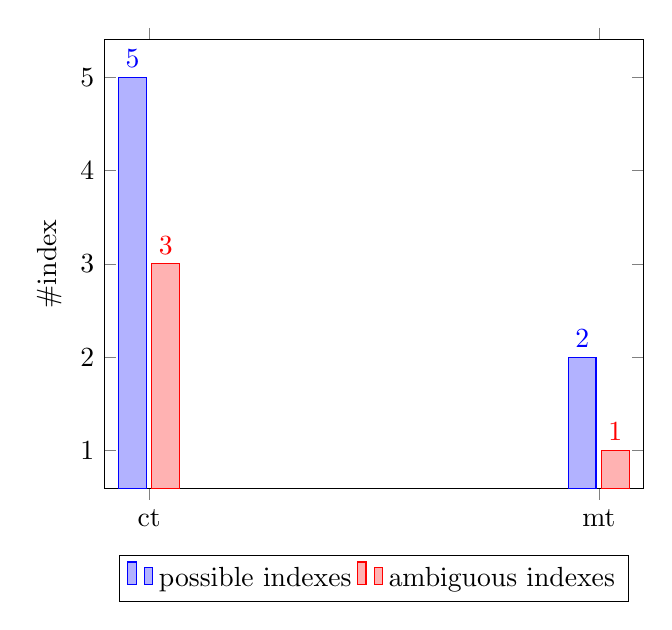
\begin{tikzpicture}
\begin{axis}[
    ybar,
    legend style={at={(0.5,-0.15)},
      anchor=north,legend columns=-1},
    symbolic x coords={ct,mt},
    ylabel={\#index},
    xtick=data,
    nodes near coords,
    nodes near coords align={vertical}
    ]
\addplot coordinates {(ct,5) (mt, 2)};
\addplot coordinates {(ct,3) (mt, 1)};
\legend{possible indexes, ambiguous indexes}
\end{axis}
\end{tikzpicture}
\caption[The index selections for MariaDB and query variant 1.]{The different
  indexes selected for MariaDB and the query variant 1, the possible index
  selections --- as in those considered by the query optimizer --- are shown next to
those actually selected.}\label{fig:plot:mariadb:query1}
\end{figure}